\subsection{Characterizing Relevant Text in the Documents}




To characterize the task-relevant text found in natural language 
software artifacts (\textit{RQ1}), 
we analyze the participants' produced highlights.
We focus
our analysis on highlights participants made of natural language
text present in the artifacts---in this case English. We do not
consider highlights participants made of source code snippets or in
tables, leaving the consideration of this information to future work.



We define a \textbf{H}ighlighted \textbf{U}nit (HU) as the full sentence containing any
highlight by a participant. 
We use sentences as the unit of analysis 
because this was the most common unit considered by the participants.
That is, of the 2,463
distinct highlights created by participants, 1,777 are sentences
(72\%), 621 are portions of sentences (25\%) and 65 are combinations
of consecutive sentences (3\%). 
Thus, if a participant highlighted just a
phrase in a sentence, we consider the full sentence as an HU or if a
participant highlighted more than one portion of a sentence we still
consider the full sentence as one HU. 


\subsubsection{How much text in an artifact is deemed as relevant to a task?}
\label{cp3:ratio}



We first ask how much text within an artifact participants found as relevant to a task.
If almost all of the text is relevant then there would not be a need for
identifying text within an artifact.
Figure~\ref{fig:task-artifact-ratio} presents the ratio of relevant and non-relevant text in each type of document.
We compute the average ratio of HUs and text for each  artifact from each type of document.
We report mean of the ratio artifact-wise to prevent misinterpretations due to outliers,
i.e., a lengthy document with few HUs or a document concentrating almost all the HUs






Considering all HUs, between 1\% to 20\% of an artifact's text is considered relevant, depending on its type.
API documents have the smallest ratio of
relevant information (mean of 3\%) and for this kind of artifact,
at most 6\% of all sentences were considered relevant.
This result is not surprising as API documents may describe many API features or
methods of which only a few are likely to apply to
a particular task.
Such quantitative analysis provides further
evidence supporting qualitative research on API
documentation obstacles.
Most notably, that the structure of APIs
and boilerplate text can bloat the documentation~\cite{robillard2011field, Aghajani2019}.
Similarly, only a small portion (4\% on average) of
bug reports are considered relevant.
This result is also not
surprising as bug reports can contain long discussions encompassing
several topics~\cite{Breu2010, Rastkar2010}.
Even the kind of document with the highest
percentage of highlights, Q\&A entries with, on average, 11\%
of the sentences being relevant,
contain a substantial amount of information not relevant to a
specific task. 







\medskip
\begin{bluequote}
    \textit{Finding task-relevant information in a bug report,
    API document and Q\&A documents require filtering to less than
    a 20\% of the documents' text.}
\end{bluequote}



\begin{figure}
    \centering
    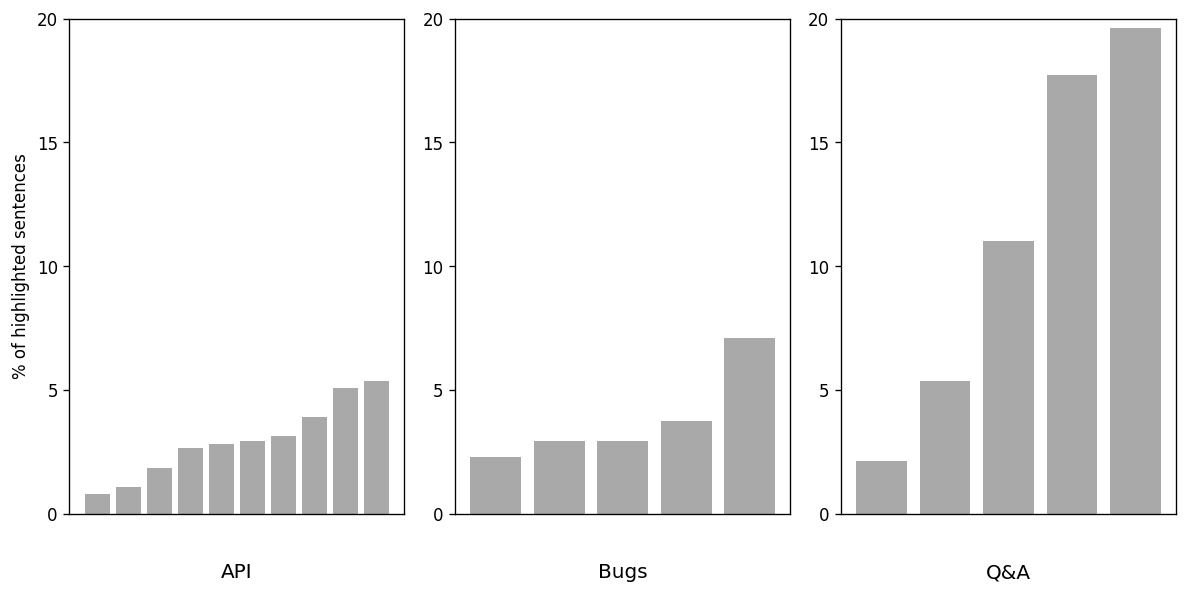
\includegraphics[width=.98\textwidth]{cp3/task-artifact-ratio}
    \caption{Percentage of highlighted sentences per artifact grouped by artifact's type}
    \label{fig:task-artifact-ratio}
\end{figure}

\subsubsection{How much agreement is there between participants about the text relevant to a task?}
\label{cp3:agreement}



To investigate the degree to which participants agree upon
the text relevant to a task, we use Nenkova and Passonneau's
pyramid method~\cite{Nenkova2004}. This method was originally used
to quantify the content of summaries produced by different annotators.
The more annotators who include the same content in their summaries,
the more consistent the view of information relevant to a summary and
the more weight given the selected content. We apply the same rationale
to assess the level of agreement of which HUs are relevant to a task
and whether agreement relates to how correctly
a participant completes a task.




To construct the pyramid, we assign a weight to each HU
corresponding to the number of participants who highlighted that HU during
a task.
Figure~\ref{fig:highlights-distribution} shows the distribution of these weights.
From the 602 HUs, we observe that 18\% of them are considered relevant by eight or more participants while 58\% are relevant to only one or two participants.
To facilitate interpreting the results,
we take into consideration how other studies provide categories for the relevance of
text (i.e.,~\cite{Petrosyan2015} and~\cite{Jiang2017}) and thus,
we aggregate levels into tiers based on the Zipfian distribution of HUs per weight~\cite{Nenkova2004}.
While aggregating levels, we preserve the observed distribution, creating a pyramid with three tiers.
Table~\ref{tbl:task-hu} presents HUs per tier.
Starting from the bottom tier, the pyramid represents the perceived relevance of information from less to more relevant.




We expect the task correctness scores of participants
to depend on how much relevant text they highlighted during the experiment.
To explore this hypothesis, we consider each HU at each tier for each task
and all scores of the participants who indicated that HU.
We then test if the number of HUs identified at each tier affects a participant's score.
As we have three independent variables (i.e., tiers) and one outcome variable (i.e., scores), we performed a multivariate analysis of variance~\cite{wohlin2012} and found significant differences ($p\text{-value} < 0.01$) between participants' score and their HUs.
We then conducted univariate tests on each tier,
finding that 
the number of HUs identified at the mid and top-tiers 
positively affect participants scores, 
what suggests that HUs from these two tiers contain key
information for completing a task.





\begin{figure}
    \centering
    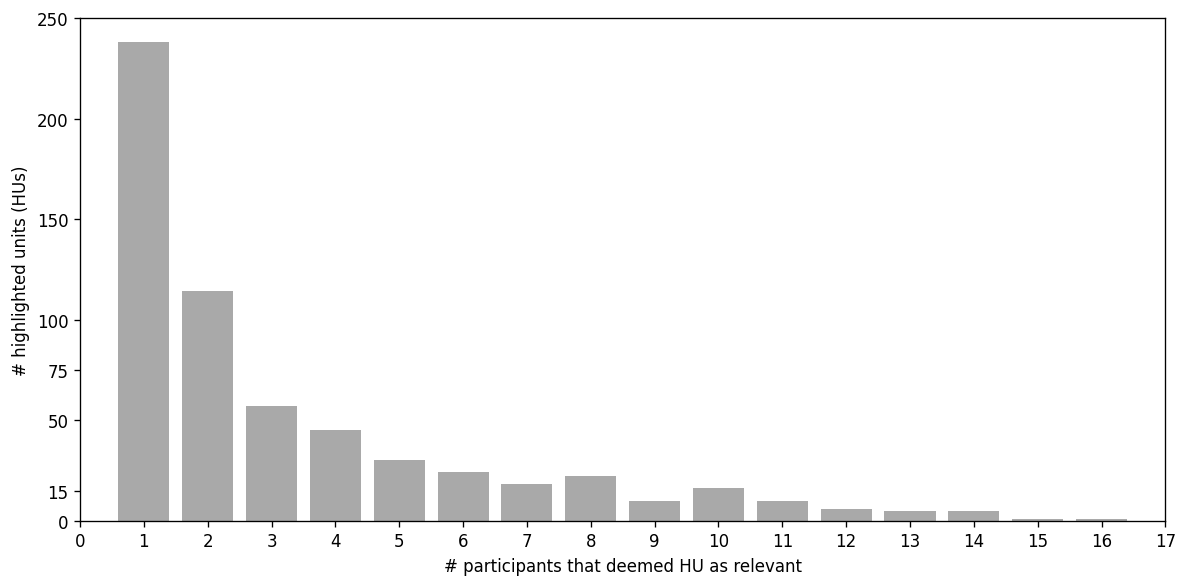
\includegraphics[width=.95\textwidth]{cp3/highlights-distribution}
    \caption{Distribution of the number of participants who deem an HU as relevant}
    \label{fig:highlights-distribution}
\end{figure}




As expected, HUs at the bottom tier vary more per participant.
We observe that there is an equal number of HUs identified by participants who successfully
completed a task and those who did not and those who report familiarity with
the technology or domain of a task and those who did not.
Due to such variability, there is no clear indication
that bottom tier HUs are from participants from a certain group, such as all those
unfamiliar with a particular technology; this is a possible explanation for the lack
of statistical significance.



\begin{table}
\begin{center}
\caption{Distribution of highlights and their respective percentages per tier for every task}
\begin{small}
% \vspace{-3mm}       
\begin{threeparttable} 
\rowcolors{2}{}{lightgray}
\begin{tabular}{l|c|cc|cc|cc}
\hline    
% Header
\textbf{Task}  
& \textbf{\# HUs} 
& \multicolumn{2}{c|}{\textbf{bottom tier}\tnote{\dag}} 
& \multicolumn{2}{c|}{\textbf{mid tier}\tnote{\dag}} 
& \multicolumn{2}{c}{\textbf{top tier}\tnote{\dag}}\\
\hline    
\hline

Gpmdpu & 43 & 23 & (53\%) & 10 & (23\%) & 10 & (23\%) \\     
Bugzilla & 103 & 51 & (50\%) & 22 & (21\%) & 30 & (29\%) \\
Yargs & 74 & 59 & (80\%) & 12 & (16\%) & 3 & (4\%) \\
Lucene & 95 & 54 & (57\%) & 24 & (25\%) & 17 & (18\%) \\
Databases & 159 & 84 & (53\%) & 41 & (26\%) & 34 & (21\%) \\
Networking & 128 & 81 & (63\%) & 37 & (29\%) & 10 & (8\%) \\
\hline    
\hline 
\rowcolor{white}
Total & 602 & 352 & 58\% & 146 & 24\% & 104 & 17\% \\

\hline 
\end{tabular}
\begin{tablenotes}
    \item[\dag] {\scriptsize The bottom tier includes HUs highlighted by 0--2 participants
    the mid tier includes HUs highlighted by 3--7 participants, and the top tier includes HUs highlight by at least 8 participants.}    
\end{tablenotes}   
\end{threeparttable} 
\end{small}
\label{tbl:task-hu}
\end{center}
\end{table}
    



\medskip
\begin{bluequote}
    \textit{Text perceived as relevant by more participants likely relates
    to key information for completing a task whereas information
    highlighted by a few participants may be more dependent on the knowledge of individuals.}
\end{bluequote}
